\documentclass[11pt,a4paper]{scrreprt}
\usepackage[utf8]{inputenc}
\usepackage[english]{babel}
\usepackage{amsmath}
\usepackage{amsfonts}
\usepackage{titling}
\usepackage{amssymb}
\usepackage{hyperref}
\usepackage{syntax}
\usepackage{listings}
\usepackage[colorinlistoftodos]{todonotes}

\newcommand{\liststy}{\small\ttfamily}

\newcommand{\fsize}{\fontsize{8pt}{10pt}\selectfont}
\newcommand{\fsizesmall}{\fontsize{7.5pt}{3pt}\selectfont\ttfamily}
\lstset{
  basicstyle = \fsize,
  identifierstyle = \fsize,
  keywordstyle = \fsize\color[HTML]{DE285F},
  keywordstyle = [2]\fsize\bfseries \color[HTML]{DE285F},
  commentstyle = \fsize\color[HTML]{839496},
  stringstyle = \fsize\color[HTML]{2429c9},
  frame=single,
  numbersep=2p,
  showstringspaces=false,
  language=sparql
}


\title{\textbf{Open Information Systems\\Final Report}}
\subtitle{2015-2016 Vrije Universiteit Brussel\\Responsible tutor : Christophe Debruyne - chrdebru@vub.ac.be}
\author{\textbf{Trackerspace}\\Matteo Marra - mmarra@vub.ac.be - 0525999 - 1M Comp Sci Soft\\Antoine Carpentier - antcarpe@vub.ac.be - 0529527 - 1M Comp Sci AI\\Titouan Christophe - tichrist@vub.ac.be - 0529190 - 1M Comp Sci Soft\\Bruno Rocha Pereira - brochape@vub.ac.be - 0529512 - 1M Comp Sci Soft}
\date{Exam Session: June 2016}
\begin{document}
\maketitle
\chapter{Introduction}
In this final report we will present our non-trivial demonstrator, \textit{Trackerspace} a web application that allows to navigate through running/biking tracks and exercise spots, that a user might use to record his workouts and look for a place where to do sport.
Our server provides a \textit{SPARQL} endpoint that can be used to query the data in our database and retrieve information according to four different ontologies, carefully linked between each other to provide a complete open information system.

We will begin describing the different ontologies we used and how we mapped to them, followed by the tools we used to develop and run our non-trivial demonstrator to finish with a description on what we achieved with our application.
\chapter{Ontologies}
\section{Ontology Engineering}
Due to the high number of students that had to take part in the realisation of the main ontology, a meeting on Slack\footnote{https://ontology-ois.slack.com} was organized. The first meeting there led, after a challenging discussion, to the first and only definition present in the ontology common to food and exercise : "A calorie is a unit of energy, it is gained by eating and lost during physical activity. A calorie equals 4.184 Joules." 

After the main ontology was defined, we all decided to split into two groups. The first group was composed of the four groups working on the \textit{exercise ontology}. The second one was working on the \textit{food ontology}. Both groups discussed their ontologies on separate channels on Slack, namely \texttt{\#exercise} and \texttt{\#food}.

Regarding the exercise group, we immediately started working on common definitions such as \textit{workout}. It was decided after a short discussion that it would be more suitable for each group to first define every one of the terms appearing in their application.  Therefore, every group shared a glossary and a diagram of their model. Another meeting was scheduled two days later to merge and adapt the definitions that would later appear in the \textit{exercise ontology}. 
During this meeting, at least one member of each group was present on the Slack channel to avoid any bias. It was implicitely decided not to have every member of each group connected in order to avoid confusion and overlapping discussions. 
We decided to proceed concept by concept, starting from a definition of \texttt{Exercise} and its properties (such as \texttt{Heart Rate}, \texttt{Equipment}, \texttt{Duration}, \texttt{Difficulty}, \texttt{Rating}, \texttt{Muscle Group}, \texttt{Repetition}).
In order to link the exercises with the global ontology, we decided to put the number of calories burned as property of an \texttt{Exercise}.

\texttt{Workout} was then defined to link an exercise session, composed by many \texttt{Exercise}, user and date.
The last concept defined during that meeting was \texttt{User} as the account of the user using the application.
At the end of the meeting, all the common entities were decided and defined.

The last meeting happened five days later in one of the computer rooms. Two members of each group were present and the ontology was ported to Webprotégé \footnote{http://starpc14.vub.ac.be:8080/webprotege/\#Edit:projectId=0f54f43f-f27d-46f0-a5bc-de5e7574ab98}. 
This operation has been done from a unique computer in order to avoid concurrency problems, with all members present to the meeting participating to this process.
In this meeting we decided that some concept we defined would refer to an already existing ontology, namely \texttt{Person}\footnote{http://dbpedia.org/ontology/Person} and \texttt{Muscle group}\footnote{http://dbpedia.org/page/Category:Muscles\_by\_location}.

Later on, during the lab session, it was decided to change \texttt{User} to \texttt{UserAccount}, linking it with a \texttt{ownedBy} property to \texttt{Person}.

The ontology was then checked via the OOPS platform and the group 3 took care of correcting all of the warnings. 

\section{Overall ontology}
%blablabla on the ontology
The non-trivial demonstrator embraces the concepts of the class ontology, called \textit{overall ontology} in this document.
As mentioned above, this ontology defines the concept of \texttt{Calorie}, defined as follows: ``A calorie is a unit of energy, it is gained by eating and lost during physical activity. A calorie equals 4.184 Joules".
\todo{insert how we mapped to it }

\section{Exercise ontology}
%blablabla on the ontology and how we mapped it
As for the overall ontology, the application follows the concepts defined in the \textit{exercise ontology} \footnote{http://starpc14.vub.ac.be:8080/webprotege/\#Edit:projectId=0f54f43f-f27d-46f0-a5bc-de5e7574ab98}, such as \texttt{Workout}, \texttt{Exercise}, \texttt{UserAccount} and \texttt{Person}. 
We encountered some differences between our application and how the ontology was defined, mainly because our application is totally different from the other applications following the same ontology. The main problem for us was that there is no concept like geographic position in the ontology, and our application is mostly based on that, since we model tracks. 

To map to the concept of \texttt{Equipment}, that is a property of an \texttt{Exercise}, we used the ID of the \texttt{Track}, since is the thing that makes more sense in the view of our application and since, choosing this solution, we wouldn't need to change too much the \textit{exercise ontology}. 
This showed us the need to create an ontology particular to our application that could map those concepts that were missing in the \textit{exercise ontology}, allowing us to relate also to the \textit{geosparql ontology} and create an end-point complete, that covers every functionality of our application.

We did not map to some concepts that, also together with the other groups in the developing process of the ontology, we reputed not necessary, such as \texttt{HearthRate} and \texttt{Repeats}.
\section{Geosparql ontology}
%blablabla on geosparql and how we mapped to it [problems we had go here?]
The OGC GeoSPARQL standard \footnote{http://www.opengeospatial.org/standards/geosparql} is a standard for representation and querying of geospatial data for the Semantic Web. It defines an ontology in \texttt{RDFS/OWL} and a \texttt{SPARQL} query interface.

It defines a class \texttt{geo:SpatialObject} and subclasses \texttt{geo:Feature} and \texttt{geo:Geometry}. It also defines a property of \texttt{geo:Feature}, called \texttt{geo:hasGeometry} that can link to a geometry.
Different types of geometries can be described, such as \texttt{Point}, \texttt{Polygon}, \texttt{Linestring} and many other.
It uses the \textit{Well Known Text (WKT)} format to serialize the different geometries.

\section{Our ontology}
%why we developed a new ontology
%the exercise ontology doesn't have any notation of position, we needed to create a new one to extend geosparql
As described in the previous sections, our ontology covers the classes and concepts that were not described in the \textit{exercise ontology}, and allow us to link our geospatial data to the \textit{GeoSPARQL ontology}, in order to increase the potential of our non-trivial demonstrator and allow to do geospatial queries on our tracks from the \texttt{SPARQL} endpoint.

In this ontology we define a \texttt{Track} and an \texttt{ExerciseSpot} that are both subclasses of \texttt{geo:Feature}. This allows to inherit the property \texttt{geo:hasGeometry}, that will be used in the mapping to the ontology to finally map the geometry of the tracks and exercise spots to the \textit{geoSPARQL ontology}.

We also define many properties like \texttt{isAlongTrack}, \texttt{hasTrack}, \texttt{performed}, \texttt{hasTags} and \texttt{hasReview}, that complete the set of data we have stored in our application.

\chapter{Tools}
\section{PostgreSQL and db2triples}
As we mentioned in earlier reports, we use PostgreSQL and PostGis to prepare our data in relational tables. The ER diagram can be found in the appendix\ref{db:er}.  We then use db2triples \footnote{\url{https://github.com/chrdebru/db2triples}} to map our entities to RDF triples. Our mapping is written in the r2rml language \footnote{\url{https://www.w3.org/TR/r2rml/}}, using the Turtle syntax. The mapping file is called \texttt{r2rml.ttl}.
%brief on db2triples, problems we had mapping to the geosparql

\section{Parliament}
Finally, we use Parliament \footnote{\url{http://parliament.semwebcentral.org/}} as our triple store. Parliament provide an indexed triples database, a web based data explorer, and a SPARQL endpoint which notably supports the geographical functions, needed to perform geospatial querying. Our demonstrator uses Parliament's SPARQL endpoint.

\section{Some issues we encounterd with the tools}
\subsection{Conversion to WKT format}
We spent some time trying to convert the geometries stored in PostGIS to WKT litterals using r2rml functions in db2triples. We also tried to make our triples using the GeoTriples \footnote{\url{https://github.com/LinkedEOData/GeoTriples}} tool. After many unsuccesful attempts, we finally found an easier way to it, using PostGIS. Using the \texttt{ST\_AsText} function, we convert the data to the Well Known Text format in the database query, and db2triples only copies it as a string in our triples. Since our specific ontology defines tracks and exercices spots as \texttt{geo:Feature} subclass, all the reasoners that might use our dataset will use those objects as geometries.

\subsection{Coordinates order in geometries}
Our initial dataset, provided in a previous iteration, included geographical data where coordinates where given in the format \texttt{latitude, longitude}. However, as we did not pay attention to this aspect before, other GIS applications and libraries use the format \texttt{longitude, latitude}. Therefore, in our first trials to query our dataset in SPARQL and display it on a map, we encountered bugs, such as erronated track lengths and tracks not found in a certain bounding box. We then converted our dataset to the \texttt{longitude, latitude} format to fit the GIS ontology.

\subsection{Elevation}
Our dataset also include elevation of the tracks, which are therefore stored as \texttt{LINESTRING Z} GIS types. Our first trials with GeoSPARQL queries didn't return any results, and we found out that projecting tracks in 2 dimensions (using PostGIS \texttt{ST\_Force2D} function in the mapping query) fixed the problem. We didn't have much time to investigate wether we could do it in GeoSPARQL or not. Also, the javascript library we use to convert geometries from WKT to geojson in our demonstrator, Wellknown.js \footnote{\url{https://github.com/mapbox/wellknown}}, does not support 3D geometries.

\chapter{Non trivial demonstrator}
\section{The application}
Our demonstrator provides an interface with a map\footnote{http://leafletjs.com/} where users are able to see all tracks in the displayed area, as well as the exercises spots along these tracks. The users are also able to find tracks by activity type. Moreover, given a track, a user will be able to find related exercises: exercises spots along the track, crossing or nearby tracks, or similar tracks by activity type or tags.

These functionalities can be found on buttons placed on the upper left of the map as buttons. The first button displays all the tracks that fit in the current shown map. The second one queries all the tracks that have at least once been used for biking and displays all of them on the map. The third and last button displays all the exercise spots on the map.

Clicking on a track gives the user more queries to do. When a user selects a track, its URI is shown and 4 buttons appear. The user can then choose to either display all the intersecting tracks, the exercise spots related to it, all the exercises that involved that track as well as the tracks the share similar particularities(e.g. tags). 

\section{Queries}
Once the query endpoint\footnote{http://openis.ititou.be:8080/parliament/sparql} was set up, different queries were written in order to display the data on the map. These queries will be explained in this section. 

The query \ref{query:alltracks} is pretty straightforward. It simply queries the triple store in order to fetch all the geometric data for all the tracks.

The query \ref{query:tracksinbox} is a little bit more complicated. It takes arguments, which are in our application the boundaries of the map and then fetches all the tracks with the condition that the tracks are contained in the boundaries defined.

The query \ref{query:trackscrossing} uses the geosparql function \texttt{sfIntersects()} in order to get all the tracks that have an intersection with the specified track. This would allow a user to, for example, know where he can change track.

Another useful piece of information a user would need is how to find tracks close to a particular place (e.g. his workplace or home). This is achieved by the query \ref{query:tracksbiking}.

The last type of query we used as an example allows us to get all the tracks that have been used for a particular activity. Query \ref{query:tracksbiking} shows an example for the biking activity.





%description on what we achieved
\chapter{Conclusions}
The non-trivial demonstrator we created satisfies all the functionalities planned. 
It is a simple web interface that allow to navigate between different tracks in different ways. Thanks to the use of \textit{geoSPARQL} all the data is consistent with the geospatial format.

We had some issues mapping to the exercise ontology, mainly because our application is totally different from the other applications of the other groups, but in the end we managed to find a coherent mapping that still saves all our functionalities.
The decision to create a new ontology allowed us to extend \textit{geoSPARQL}, and so to get all the benefits of its classes and queries, other than \textit{opening} our information system not only to the class ontology.

Overall, this was a really interesting project to develop. 
It was not so difficult but still challenging to find an agreement between different groups in the class, because, even if the domain was the same, the applications have many differences between each other.
It was also really interesting to work with \textit{geoSPARQL}, even if sometimes the documentation is lacking, slowing down the development of the queries.


\chapter*{Appendix}
\begin{lstlisting}[caption={Prefixes used in the hereinbelow queries},label=query:prefixes]
PREFIX geo: <http://www.opengis.net/ont/geosparql#>
PREFIX geof: <http://www.opengis.net/def/function/geosparql/>
PREFIX rdf: <http://www.w3.org/1999/02/22-rdf-syntax-ns#>
PREFIX sf: <http://www.opengis.net/ont/sf#>
PREFIX exont: <http://webprotege.stanford.edu/ontologies/ExerciseOntology#>
PREFIX ont: <http://openis.ititou.be/ont#>
PREFIX tr: <http://openis.ititou.be/ont#>
\end{lstlisting}
\begin{lstlisting} [caption={Query for all tracks},label=query:alltracks]
SELECT DISTINCT ?track ?geom
WHERE {
    ?track rdf:type tr:Track.
    ?track geo:hasGeometry ?geom.
}
\end{lstlisting}

\begin{lstlisting} [caption={Query for tracks in a defined box},label=query:tracksinbox]
SELECT DISTINCT ?track ?geom
WHERE {
  ?track rdf:type tr:Track.
  ?track geo:hasGeometry ?geom.
  FILTER (
    geof:sfContains(
      STRDT("POLYGON((${lon1} ${lat1}, 
      				  ${lon1} ${lat2}, 
      				  ${lon2} ${lat2}, 
      				  ${lon2} ${lat1}, 
      				  ${lon1} ${lat1}))", 
      	    sf:wktLiteral),
      STRDT(?geom, sf:wktLiteral)
    )
  ).
}
\end{lstlisting}

\begin{lstlisting} [caption={Query for tracks having an intersection with a specified track},label=query:trackscrossing]
WHERE {
  ?track rdf:type tr:Track.
  ?track geo:hasGeometry ?geom.
  <${track}> geo:hasGeometry ?x.
  FILTER (
    geof:sfIntersects(
      STRDT(?x, sf:wktLiteral),
      STRDT(?geom, sf:wktLiteral)
    )
  ).
}
\end{lstlisting}
\pagebreak
\begin{lstlisting} [caption={Query for tracks used at least once for biking},label=query:tracksbiking]
SELECT DISTINCT ?ex ?track ?geom
WHERE {
    ?ex rdf:type exont:Exercise.
    ?ex exont:HasType "Biking".
    ?ex ont:hasTrack ?track.
    ?track geo:hasGeometry ?geom.
}
\end{lstlisting}

\begin{lstlisting}[caption={Query for tracks within a specified distance of a point }, label = query:tracksbiking ]
SELECT DISTINCT ?track ?geom ?dis
WHERE {
    ?track rdf:type ont:Track.
    ?track geo:hasGeometry ?geom.
    LET (?dis := geof:distance( 
    				STRDT(?geom, sf:wktLiteral), 
    				STRDT("POINT(4.15 51)", sf:wktLiteral),
    				uom:metre)).
    FILTER(?dis < $(dist)).
}
\end{lstlisting}

\begin{lstlisting}[caption={Query for tracks with a tag common with a specified track }, label = query:tracksbiking ]
SELECT DISTINCT ?track ?geom
WHERE {
    ?track rdf:type ont:Track.
    ?track geo:hasGeometry ?geom.
    <${track}> ont:hasTags ?tag.
    ?track ont:hasTags ?tag.
\end{lstlisting}

\begin{figure}[h]
    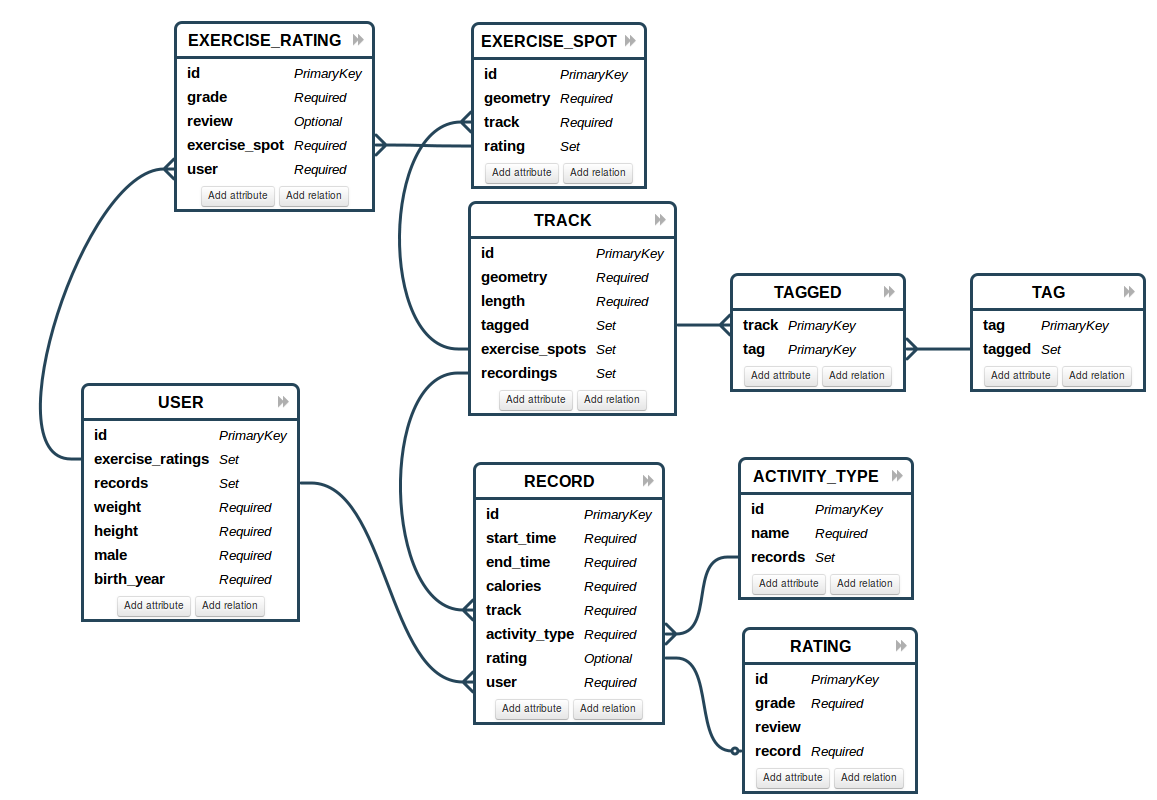
\includegraphics[width=\textwidth]{er-diagram.png}
    \caption{Entity Relationship diagram}
    \label{db:er}
\end{figure}

\end{document}